\documentclass[nobib]{MSword}
% Class options:
%-------------------------------
% nobib         - skip bibliography code/ don't include bib
% math          - include math packages and useful math commands
% hidelinks     - hide hyperref colored link boxes
% wordlinks     - link color scheme similar to word


% Preamble code:
%%%%%%%%%%%%%%%%%%%%%%%%%%%%%%%%%%%%%%%%
\usepackage[english]{babel}
\usepackage{csquotes}
\usepackage{lipsum}

% % Uncomment using "Ctrl + /" (/ on numpad):
% % Customizing headers and footers:
% \fancypagestyle{custom}{%
%     \fancyhf{}% clears the footer and header
%     % Header:
%     \fancyhead[L]{}
%     \fancyhead[C]{}
%     \fancyhead[R]{}
%     % Footer:
%     \fancyfoot[L]{}
%     \fancyfoot[C]{}
%     \fancyfoot[R]{}
%         % Tips:
%         % ----
%         % L: left, C: center, R: right
%         % O: odd pages, E: even pages
%         % ----
%         % Example: \fancyghead[LO,RE]{Text}
%         % will produce "Text" left in the header
%         % on odd pages and right in the header on even pages.
%     % Rules/ lines:
%     \renewcommand{\headrulewidth}{0.4pt}
%     \renewcommand{\footrulewidth}{2pt}
% }
% % Changing the pagestyle:
% \pagestyle{custom}

%%%%%%%%%%%%%%%%%%%%%%%%%%%%%%%%%%%%%%%%

% Preamble information:
%%%%%%%%%%%%%%%%%%%%%%%%%%%%%%%%%%%%%%%%

\title{Step and Impulse Response of a RLC Band Pass Filter}
\author{Dre Mata}
\date{19 Feburary 2023}

%%%%%%%%%%%%%%%%%%%%%%%%%%%%%%%%%%%%%%%%

% The document:
%%%%%%%%%%%%%%%%%%%%%%%%%%%%%%%%%%%%%%%%
\begin{document}

\maketitle
\begin{center}
    Part 1:
\end{center}
 The objective of part one is to plot the impulse response of the RLC Band Pass Filter circuit using functions created by hand and the build in scipy.signal.impulse() function. The first task is to plot the functions from the prelab calculations. This can be seen in Figure one. The next task in part one is to use the scipy.signal.impulse() to plot the transfer function from the prelab. This can be seen in Figure two.


\begin{center}
    Part 2:
\end{center}
The objective of part two was to use the scipy.signal.step() function to plot the transfer function of H(s) and to use the final value theorem to show that the transformation was done properly. The first task is to use the scipy.signal.step() function to plot the step response. This can be seen in Figure three. The next task was to use the final value theorem to show the transformation was done properly. This can be seen in Figure four. The results from figure two make sense with out results in figure four, because the plot in figure two is at zero at time infinity. The plot in Figure three is at zero at time zero.

\begin{center}
    Questions:
\end{center}
1. Explain the result of the final value theorem from Part 2 Task 2 in terms of the physical circuit components.

The final value theorem says that the limit of the impulse function as time approaches infinity is equal to the limit of the transfer function multiplied by s as time approaches zero. For the first part of this theorem we see that the impulse function approaches zero as time goes to infinity. This makes sense, because In the RLC circuit the voltage will keep oscillating because of the inductor and capacitor, but will loose voltage due to the resistor. So over time the voltage will go to zero. For the second part of the final value theorem the transfer function being zero at time zero makes sense, because the circuit it about to be turned on. This can be through of as flipping a switch.

\begin{center}
    Figures
\end{center}

Figure 1:

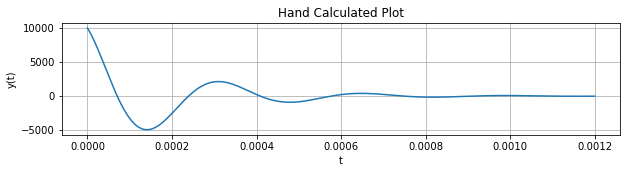
\includegraphics[scale = 0.50]
{txt/Lab5Fig1.png}

Figure 2:

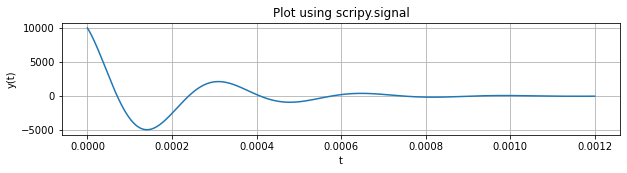
\includegraphics[scale = 0.75]
{txt/Lab5Fig2.png}

Figure 3:

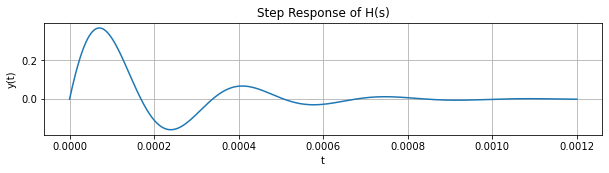
\includegraphics[scale = 0.75]
{txt/Lab5Fig3.png}

Figure 4:

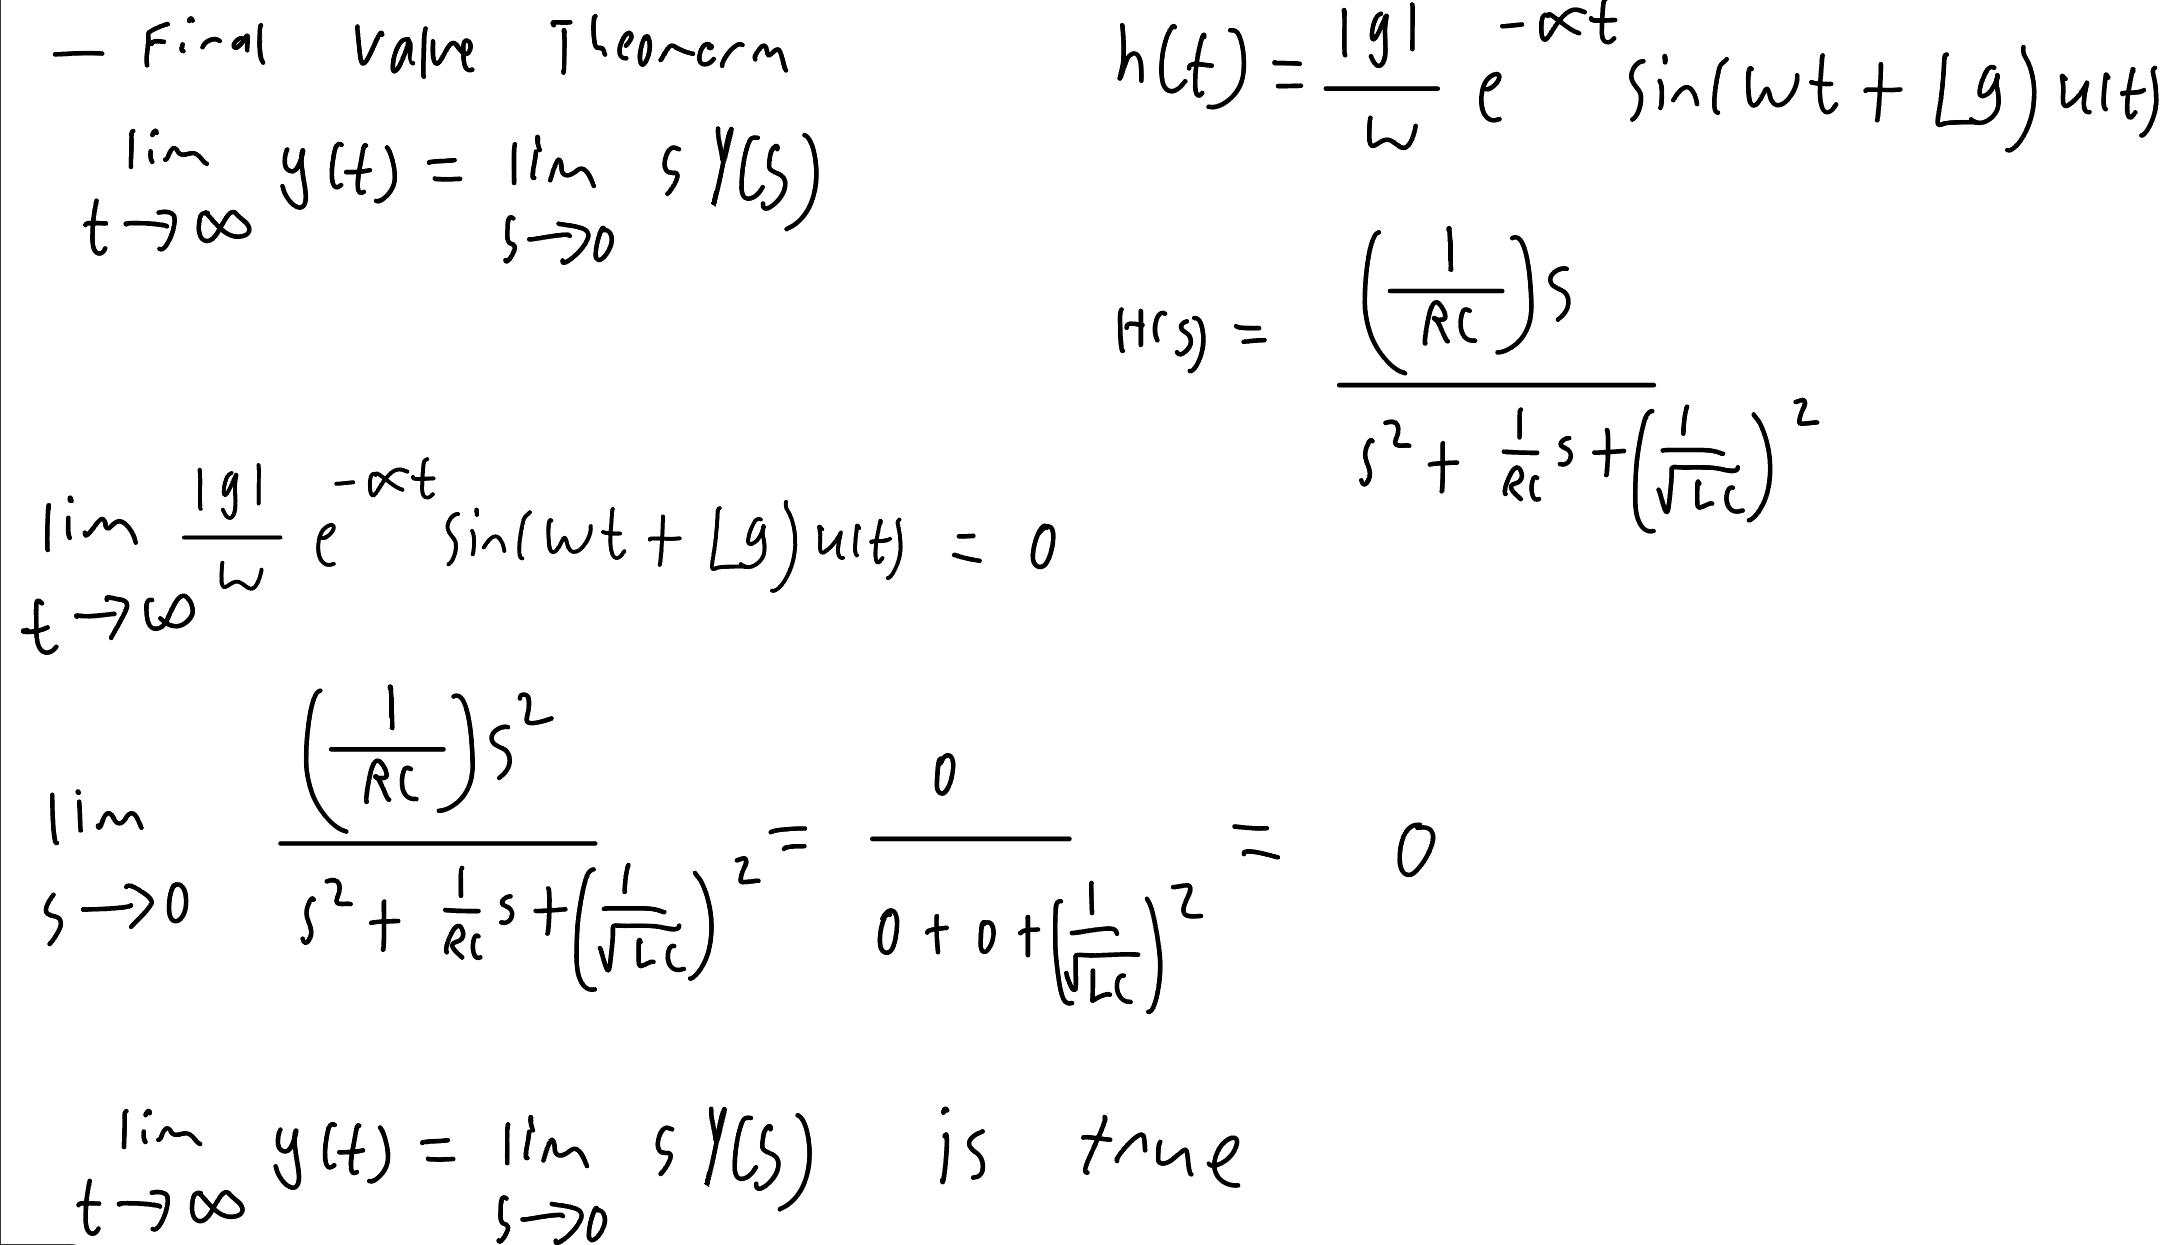
\includegraphics[scale = 0.2]
{txt/Lab5Fig4.jpeg}

\begin{center}
    Conclusion
\end{center}
This lab helped me gain a better understanding of some of the functions that python has. In doing this I gained some valued insight on RLC circuits and how the voltage within them acts of a period of time. Also how the Laplace transform can be used to find the relationship of voltage and time by solving a differential equation.
\end{document}

%%%%%%%%%%%%%%%%%%%%%%%%%%%%%%%%%%%%%%%%

% Copyright Remarks:
%--------------------

% Copyright holder: Vebjørn S. Førde, copyright: CC BY 4.0
% Note: The author of this template is also the copyright holder.

% Below is an explanation of the CC BY 4.0. Additional statements/ 
% clarifications made by the author/copyright holder are marked with *.

% YOU ARE FREE TO:
% Share — copy and redistribute the material in any medium or format
% Adapt — remix, transform, and build upon the material
% for any purpose, even commercially.

% UNDER THE FOLLOWING TERMS:
% Attribution* — You must give appropriate credit, provide a link to the license,
% and indicate if changes were made. You may do so in any reasonable manner, but 
% not in any way that suggests the licensor endorses you or your use.

% *Note: 
% Attribution NOT NEEDED for: 
%       - PDF distibution (like sharing your PDF document)
%       - Use of (dummy)text and images provided in the template (obviously)
%       - Distributing parts of the template, and not the template as a whole
% I am not really concerned with being given credit. As long as you do not 
% claim to have made the template yourself in distributing it further, I have
% no complaints.

% No additional restrictions — You may not apply legal terms or technological 
% measures that legally restrict others from doing anything the license permits.

% NOTICES:
% No warranties are given.

% Disclaimer* (added by copyright holder):
% THE SOFTWARE IS PROVIDED "AS IS", WITHOUT WARRANTY OF ANY KIND, EXPRESS OR
% IMPLIED, INCLUDING BUT NOT LIMITED TO THE WARRANTIES OF MERCHANTABILITY,
% FITNESS FOR A PARTICULAR PURPOSE AND NONINFRINGEMENT. IN NO EVENT SHALL THE
% AUTHORS OR COPYRIGHT HOLDERS BE LIABLE FOR ANY CLAIM, DAMAGES OR OTHER
% LIABILITY, WHETHER IN AN ACTION OF CONTRACT, TORT OR OTHERWISE, ARISING FROM,
% OUT OF OR IN CONNECTION WITH THE SOFTWARE OR THE USE OR OTHER DEALINGS IN THE
% SOFTWARE.

% Read more about CC BY 4.0:
% https://creativecommons.org/licenses/by/4.0/